% Survey of existing FPGA-based discrete event simulators, and their
% microarchitectural design.

For the purpose of this dissertation, it is insightful to classify FPGA-based
RTL simulators along two dimensions. For simplicity, here we consider only
single-FPGA hosts, but we note that this discussion can trivially extended to
multi-FPGA hosts. This chapter was heavily influenced by dicussion in Pellauer
and Vijayaraghavan et al. in \emph{A-Port Networks: Preserving the Timed
Behavior of Synchronous Systems for Modeling on FPGAs}~\cite{APortNetwork}.

The first dimension, is timekeeping strategy. \emph{Explicit timekeeping}~(ET)
simulators, keep track of simulation time whereas simulators with implicit
timekeeping (IT) instead rely on target-cycle count as a proxy for target time. This represents an
implementation optimization, as additional FPGA resources required track and
manage timestamps are unneeded. For this optimization to apply broadly across
the simulator, target system clocks must have fixed frequency and phase, and
all simulation events must be synchronous to these clocks.

The second dimension is control granularity. At one extreme there exist
simulators with \emph{centralized control} (CC). These track time in
a single location, the entire simulator advances in lockstep from
timestep to timestep.  Conversely, there are simulators with \emph{distributed
control}~(DC). These simulators are parallel systems of \emph{logical
processes}~(LP). Each LP locally tracks simulation time and can advance
independently. DC simulators can be coarse-grained, with a logical process
simulating core-scale components of the SoC, core of the SoC, or fine-grained,
herewit logical processes may take on the scope of a CAM, RAM, or even a
combinational circuit like a multiplexer.

Taking the product of these two dimensions produces four classes of simulator:

\begin{enumerate}
\item{Implicit Timekeeping, Centralized Control (ITCC)}: Simple MIDAS generated simulators*. FabScalar FPGA

\item{Implicit Timekeeping, Distributed Control (ITDC)}: RAMP simulators,networked MIDAS-generated simulators.

\item{Explicit Timekeeping, Centralized Control (ETCC)}: Unrealized, commerical emulators*. Example: Direct implementations of the verilog event queue.

\item{Explicit Timekeeping, Distributed Control (ETDC)}: Multi-FPGA commerical emulators*, This Work
\end{enumerate}

It is critical to note DC simulators are in effect FPGA-hosted, parallel
discrete-event simulators.  Parallel, discrete-event simulation~(PDES) has been
a vibrant area of research since the 1980s, but PDES researchers have focussed
nearly exclusively on non-FPGA hosts (including multiprocessors, GPUs,
supercomputers, networks thereof).  In the next sections, we briefly introduce
relevant PDES work, and explain how prior work in that field translates to
hosting DC full-system simulators on FPGAs. First, we explore some
CC simulator designs to help motivate the additional complexity DC simulators incur.

\section{An Iron Law For FPGA-Based Simulator Performance}

If SoC designers turn to hardware emulators for speed, it is critical
to understand how emulator design affects throughput. For IT simulations of a target
with a single clock domain, Pellauer et al. present a simple performance
equation, which like the iron-law of processor performance that inspired it,
breaks down the performance of a complete simulation into a product of terms:

\begin{equation}
    f_{sim} = \frac{cycles_{t}}{cycles_{h}} f_{fpga}
\end{equation}\label{eq:sim-perf}

\noindent Where,
\begin{flalign*}
    f_{sim} &= \text{throughput of the simulator (target cycles per second, Hz)}\\
    f_{fpga} &= \text{the clock frequency of the host FPGA (Hz)}\\
    cycles_{h} &= \text{the total number of host cycles over which the simulation executed}\\
    cycles_{t} &= \text{the total number of target cycles simulated}\\
\end{flalign*}

The right term of this equation, host frequency~($f_{fpga}$), is set by the
critical path delay of the simulator. Depending on the simulator's design, and
the target it models, this may sometimes be SoC RTL often corresponding to a
critical path in the actual implementation, but more likely, it is a path that
drives scheduling logic in the simulator itself (i.e., deciding whether to
advance forward in simulation time or fire a target clock edge).
The left term, a ratio of host-to-target cycles is a measure of the
microarchitectural efficiency of the simulator. In an FPGA prototype, this term is
effectively unity: every host clock simulates a target clock. In
a host-decoupled simulator, in practise, it is always less than one\footnote{While it is possible to simulate multiple target cycles per
host cycle by unrolling successive cycles of execution, there is no incentive
to do so globally across a simulator, as it would double resource utilization,
and likely double the critical path length of the simulator. In DC simulators
of target machines with multiple clock domains, it may make sense to do this
for relatively small LPs in the fastest clock domains, if the simulator is
rate-limited on those LPs.}. Given this, Pellauer et al. tend to the
more-intuitive recipricol of this term and call it FPGA-cycles-to-Model-cycles
Ratio~(FMR). We give it below.

\begin{equation}
    FMR = \frac{cycles_{h}}{cycles_{t}}
\end{equation}\label{eq:fmr}

As an example, consider a 5-read, 3-write register file modelled by an LP that
uses a 2-ported block RAM. If the LP statically schedules all 8 accesses, it
will have an FMR of 4. Conversly, a more clever design that dynamically
schedules accesses only if the ports are used could have lower FMR. In
simulations where the register file is lightly used the FMR of the LP could
approach unity, whereas when it is heavily used it would approach the static
limit of 4. Unless it is statically defined, FMR can only be usefully defined
as an average over the execution of a particular simulation. Continuing with
this example, one could gang-together multiple BRAMs or LUTRAMs to build a more
highly-ported RAM structure that could model more port accesses per cycle.
While this could reduce the statically scheduled FMR from 4 to as low as 1, it
comes at the expense of FPGA resources and, potentially, longer simulator
critical path adversely affecting the second term of \ref{eq:sim-perf}.

For this to apply to DC simulators, we can modify the equation above to use the FMR of
the LP that has executed the fewest number of target cycles in the system. We
note though, that when LPs may advance only a bounded number of cycles ahead of
slower LPs in the system for sufficiently long simulation, the equation above
returns approximately the same result for all LPs.

\section{Centrally Controlled~(CC) Simulators}

It is natural, when first building a simulator, to attempt to coordinate time
globally across the FPGA. It is simpler to implement; there are fewer potential
sources of causality errors, as there aren't different pieces of the simulator at different points in simulated time; and it is considerably
easier to capture snapshots of the simulated system at particular points in
time. In a system where different components of the target may take different,
or even dynamically changing number of host cycles to model, there are two
common approaches.  The first, is what A-Port Networks, as \emph{Unit-Delay
Simulation}. Here the simulator is granted a fixed $N$ host-clock-cycles to
compute each target-cycle, where $N$ is selected to equal the largest possibly
latency a sub-block may take to model its piece of the target~(its FMR is $N$). While simple to
implement, this will result in lost host-cycles, if in some target cycles the
full $N$ cycle allocation is unneeded.  We also note that while it's
relatively easy to provide tight bounds for models of many on-chip
blocks it may be more difficult for I/O devices, which may require large $N$
in the worst case, but far less on average.

A natural optimization to make, is to allow sub-blocks to signal when they have
finished computing.  The centralized controller aggregate done-signals from all
blocks in the system and steps the simulator only once all have been
asserted~(i.e., a wide and-reduction).  This is called \emph{Dynamic-Barrier
Synchronization}. While this removes wasted host idle cycles (FMR can fall
below $N$), it introduces new control signals that must be routed to a central
location on the FPGA. This adds considerable wire delay to paths that likely
lie on the simulators critical path. This problem is exacerbated in modern
FPGAs, like the VU9P devices used in EC2 F1, which are composed of multiple
dies~\footnote{In Xilinx parlance, each logic die is referred to as a
super-logic regions~(SLRs).}, as these control signals must use relatively
scarser and higher-delay inter-die interconnect. Additionally, the scarcity of inter-die interconnect
puts increased pressure on the router, and for high utilizations often results
in unrouted nets, and other related DRC errors.  To improve simulator
frequency, it is natural, perhaps even necessary, to pipeline these signals at
the expense of a fixed increase to FMR: unless simulation of target cycle can
be overlapped, FMR will increase by 1 for each additional pipeline stage. While
FPGAs have scaled in capacity, their logic delays, and thus achievable
$f_{max}$, have seen little improvement. This increase in capacity begets a
greater number of units, increasing the number of terms in the and-reduction
network and lengthening critical path of the simulator.

These trends in FPGA scaling make it natural to want to decentralize
timekeeping in the simulator.  Having more LPs, each of which have to manage a
fewer number of control signals, that are routed more locally, should improve
${f_{fpga}}$ while easing the routing and DRC challenges with centralizing
control.

\section{Software PDES}
Software PDES can be divided into two classes based on how they address
deadlock.  In \emph{Conservative} PDES, logical processes issue messages
non-speculatively, as a result, an output message that \emph{may} depend casually on a
particular input message will not be issued until that input arrives.
Conservative PDES addresses deadlock by requiring LPs to have non-zero
\emph{lookahead}. That is to say, output messages must only depend on input
messages that are at least  $t_{lookahead}$ seconds in the past. In order to gaurantee forward
progress, if a logical process is blocked on a particular input, whose latest
message is timestamped to time $t_{i}$, it can and must eventually issue a
\emph{null-message} at time $t_{i} + t_{L}$ on it's output channels. Supposing
the blocked, path does not contain a cycle of LPs no lookahead, the simulation
will advance.  Large lookahead improves simulation performance, as the number
of null-messages required to avoid deadlock increases as lookahead approaches 0.
In general, lookahead is derived from underlying properties of the system under simulation;
if sufficient lookahead cannot be captured in the underlying system, conservative PDES algorithms may
offer little benefit over sequential simulators.

The second class PDES simulation are \emph{optimistic}. Optimistic deadlock
avoidance first was presented in the Time Warp~\cite{TimeWarp}. In optimistic
pdes, lps send messages speculatively. Necessarily, LPs have mechanisms to
rollback from misspeculation and to inform downstream LPs of earlier messages
that were erronously sent. In Time Warp, LPs correct for mispeculated messages,
by sending \emph{anti-messages}, which as the physics-analogy would suggest,
\emph{annihiliate} its corresponding pair-message that was erronously sent previously.

Though a conservative vs. optimistic PDES debate raged through
the 90s and 00s, both optimisitic and conservative PDES algorithms see
contemporary use.
- Summary of where they are used.

\subsection{Considerations for FPGA-Hosted PDES}

FPGA are a unique host platform relative to those studied in the PDES
literature, as a number of complications introduced by multiprocessors and
networked-hosts do not apply. Notably:

\begin{enumerate}
\item{FPGAs trivially support FIFO communication channels}. Unlike in
conventional PDES hosts, channels between FPGA-hosted LPs are easily made FIFO.
In a conservative PDES implementation, LPs do not need to reorder messages, and
can assume messages from the same sender arrive in monotonically increasing
time-order.

\item{Transmissions errors are rare}. FPGA-hosted channels (i.e., hardware
queues) operate reliably, and even those that cross asynchronously related host-clock-domains
can be made to operate such that LPs do not need to tolerate potentially lost messages.
\end{enumerate}

The major challenge FPGA-hosts introduce over their CPU-host counterparts is
that many of the state-of-the-art PDES algorithms are complex, making
them a challenge to implement in hardware and expensive to support in FPGA
fabric. At least one general-purpose, FPGA-hosted PDES has been built: PDES-A~\cite{PDESA}~\cite. PDES-A
implements an optimistic algorithm, over an array of processing elements~(PEs).
While it would be possible to implement RTL simulator using
PDES-A, the effective simulation capacity and throughput of such a system would be
considerably lower than FPGA-based emulators. ASIC emulation aside, it is
reasonable to assume that likely some domain-specific, FPGA-hosted PDES have been built
and published in their respective fields. One example published at FCCM by
Herboldt et. al.~\cite{MolecularFPGAPDES} to simulate molecular dynamics.
% See PDESA paper for cite

\section{ASIC Emulation As Domain-Specific PDES}

In effect, DC simulators are domain-specific, FPGA-hosted PDES for doing ASIC emulation.
As an application domain, ASIC emulation has a number of properties that make FPGAs well-suited for one another:

The first, most obvious reason is the reason FPGAs are used as ASIC prototyping
platforms, they are a good implementation substrate for LPs. In the case of a RTL block with a single clock, a
simple LP implementation clock-gates the block it models, and adds one or more state
machines to control when to fire the clock, and enqueue and dequeue messages
from other LPs. When an LP clock fires, what would be thousands, possibly
millions or billions, of events in a software simulator is computed
concurrently in a single host cycle. We expand on various LP implementations in
the next section.

Second, since FPGAs offer high-bandwidth, and critically, low-latency
interconnect between LPs that is tailored to the target, it is possible to
decompose an ASIC into closely-coupled LPs that synchronize on a per-cycle
basis. High bandwidth interconnect between LPs removes any need to compress, or
otherwise optimize, transmission between LPs, reducing simulator complexity.
Hundreds, even thousands, of cycle-by-cycle traces of messages can be trivally
moved between LPs on the same FPGA, a feat that is all but impossible to
achieve on a CPU host. LPs can be directly connected to one another with
hardware queues, which in the general case, have a single host cycle of
"transmission" delay. In some cases, flow-through queues or wire connections
may be used to allow combinational transmission of messages. This permits
decomposing an ASIC into LPs that are closely, even combinationally, coupled in
the target, without grossly affecting simulation performance.

If you accept that FPGAs appear to be good hosts of PDES for ASIC emulation,
the next question becomes how does one translate an ASIC into a graph of
logical processes, which given a set of restrictions on their behavior, avoid
deadlock, preserve the behacior of the source RTL, while still mapping
efficiently onto the FPGA. We refer to the set of rules that define the
behavior of these graphs as a \emph{target formalism}.  As you will see,
properties of these graphs exploit features of the underlying target to permit
building conservative PDES that statically avoid deadlock, and so do not need
to employ any dynamic mechanisms for avoiding or resolving it. % Citations
These formalisms permit building ad-hoc simulators, where a designer manually
writes LP implementations that they stitch together to model a target design
that has not yet be built, or hardware emulators, where the graph is inferred by a compiler that is processing extent SoC RTL. In
the latter case, not only can LP implementations be shown to adhere to the
rules of the target formalism, but it's simulated behavior can be verified
against the source RTL to show it maintains the same timed behavior.

\section{Target Formalisms}

Target formalisms for ASIC emulation generally can be defined by a tradeoff
between simulation performance and modelling flexibility. More flexible
formalisms lift restrictions on LP definition and permit tighter coupling
between LPs, enabling finer-grained resource optimizations. We explore three
formalisms: the RAMP model, APortNetworks, and LI-BDNs. One common feature of
all three formalisms is that they are designed to support conservative, IT
simulators: messages are not timestamped, and LPs transmit new messages to all
of their neighbors for every target cycle. Having a fixed-interval between
messages removes the need for conventional conservative PDES deadlock avoidance
(i.e, null messages) or detection schemes, instead deadlock avoidance in these
formalisms is provided by-construction by constraining how combinational paths
may be modelled between LPs and the conditions under which LP implementations
must enqueue and dequeue messages.

\section{Channel-Bootstrapped Formalisms}

The RAMP target formalisms and APort Networks are examples of what we define as
\emph{channel-bootstrapped} formalisms as they rely on the use of special
point-to-point LPs called \emph{channels}, in RAMP parlance, to send the
initial messages of the simulation. Channels are LPs because they
model stateful interconnect: it is this statefulness that allows them to send output
messages at time 0 before receiving any input messages.

With that said, RAMP and APortNetworks differ primarily in the granularity of
their supported non-channel LPs. The original RAMP formalism defined
non-channel LPs, called \emph{units}, at latency-insensitive boundaries in the
target. This would make blocks on the scale of cores, or DRAM controllers
reasonable candidates for definition as an LP. Naturally, channels models latency
insensitive interconnect, and generically can be defined by four parameters shown in \TODO{figure}.

In practise, it is rare to find boundaries in the target design where all
interfaces are latency insensitive, as often some subset of signals, like reset
and interrupts, are driven combinationally or through a set of register stages.

APortNetworks was designed to support finer-grained LPs that are coupled with
register stages in the target. This relaxation makes it possible to define
finer-grained LPs -- in their paper, Pelleaur et al. use a processor pipeline
as a motivating example and divide different pipeline stages into seperate LPs.
Later versions of the RAMP architecture, introduced the same sort of channel,
called a \emph{pipe-type} channel, shown in \TODO{Figure}

Pipe channels are defined by a single parameter $l$, corresponding to their
latency. Assuming the underlying registers they model are not reset
explicitly a using target signal, but are instead initialized at time 0 to some
statically known value, they may provide $l$ initial messages before they must
stall for an input message.

Neither formalism appears to give any treatment to modelling a target-driven reset in
channels, as they both rely on time-zero intialization to effectively
"reset" target state.  We note that if these underlying state elements are
synchronously reset, the channels with $l >= 1$ may provide no more than 1
initial message, afterwhich its output may causually depend on a reset
message\footnote{We further note that neither of these formalisms was designed
to support asynchronously reset as all-events are synchronous to an implicit
clock. At a first blush, however, asynchronous reset mandates that that even
the first message emitted by a pipe-channel with $l > 0$ would depend causually
on reset at time 0.}. A pipe-type channel with $l = 0$, is a degenerate LP that models a wire between the producer and consumer LP, coupling them combinationally.
It models no target state and merely relays messages from producer to consumer.

Units model a single target cycle of execution by dequeuing an input message
from each of its input ports, and enqueing a new output message into each of
it's output ports. The simplest unit implementation, and the one perscribed by
APort Networks, waits for all input messages to arrive and all of it's output
ports to be ready to accept to messages, before it may \emph{fire}. Then the
unit computes its state updates and simulateously enqueues a single output
message into each output port, and dequeues a message from each input port.
Figure~\ref{fig:adder-example} demonstrates the execution of a single target cycle in a channel-bootstrapped formalism.

\begin{figure*}
    \centering
    \begin{subfigure}[t]{0.49\textwidth}
        \captionsetup{margin=0.25cm}
        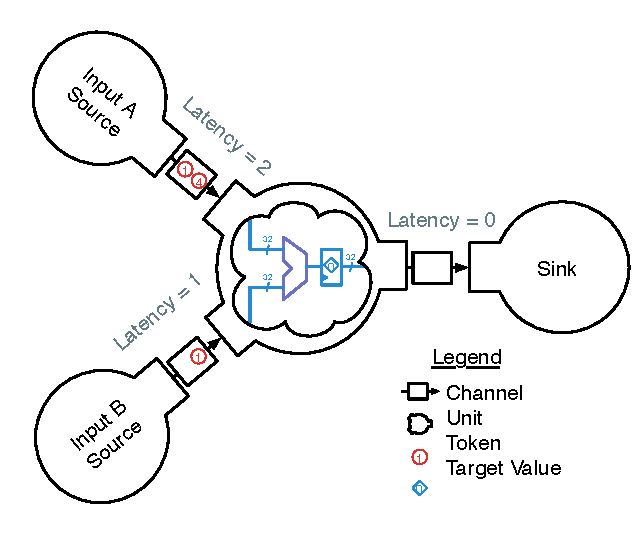
\includegraphics[width=\columnwidth]{figures/adder-example1.pdf}
        \caption{Initial state of the graph.}
        % graffle2pdf -c initial-state midas-graphics/graffle/adder-example.graffle figures/adder-example1.pdf
    \end{subfigure}
    \begin{subfigure}[t]{0.49\textwidth}
        \captionsetup{margin=0.25cm}
        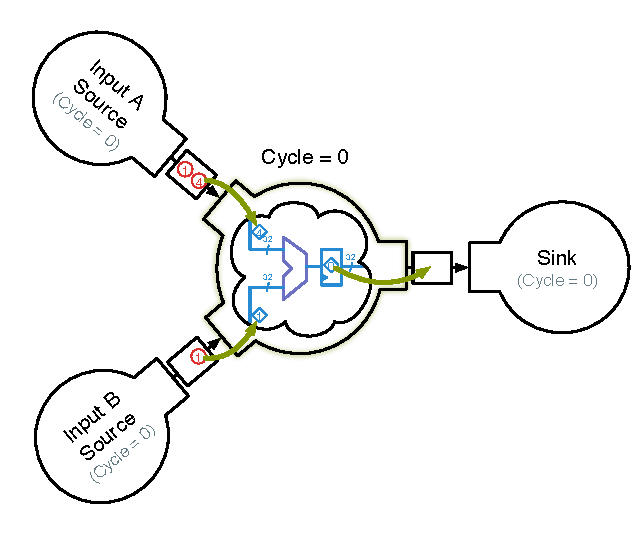
\includegraphics[width=\columnwidth]{figures/adder-example2.pdf}
        \caption{With all input tokens available, the unit fires and advances to cycle 1.}
        % graffle2pdf -c tfire-cycle0 midas-graphics/graffle/adder-example.graffle figures/adder-example2.pdf
    \end{subfigure}
    \begin{subfigure}[t]{0.49\textwidth}
        \captionsetup{margin=0.25cm}
        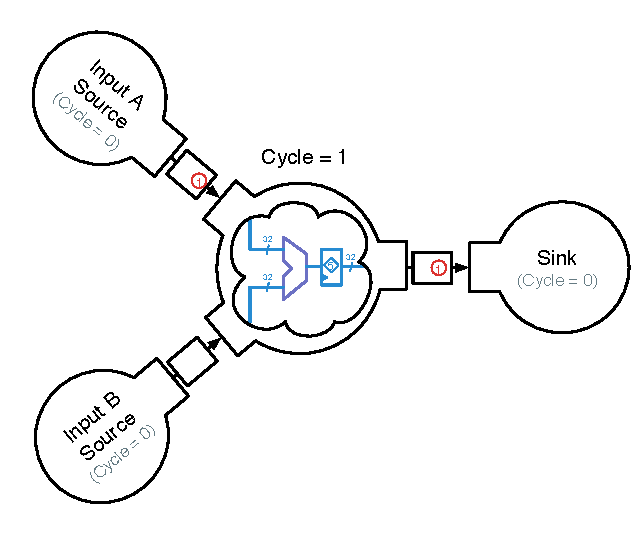
\includegraphics[width=\columnwidth]{figures/adder-example3.pdf}
        \caption{The state of the graph after firing. The unit is stalled on the arrival of a B-input token.}
        % graffle2pdf -c cycle1 midas-graphics/graffle/adder-example.graffle figures/adder-example3.pdf
    \end{subfigure}
    \begin{subfigure}[t]{0.49\textwidth}
        \captionsetup{margin=0.25cm}
        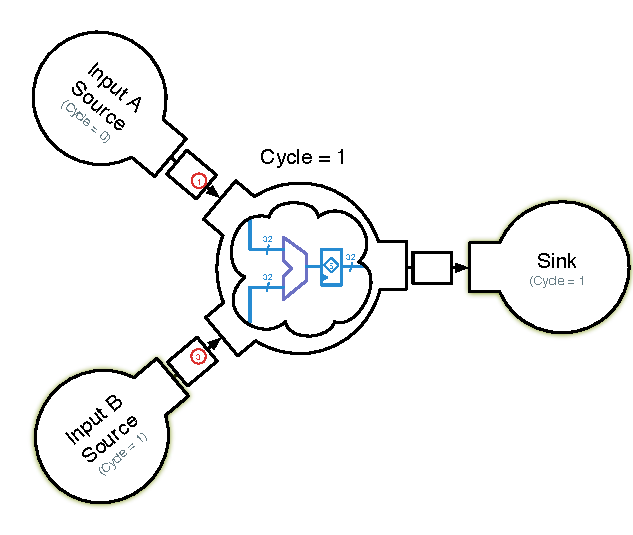
\includegraphics[width=\columnwidth]{figures/adder-example4.pdf}
        \caption{Input B source fires, producing the needed token.}
        % graffle2pdf -c inputb-fires midas-graphics/graffle/adder-example.graffle figures/adder-example4.pdf
    \end{subfigure}
    \begin{subfigure}[t]{0.49\textwidth}
        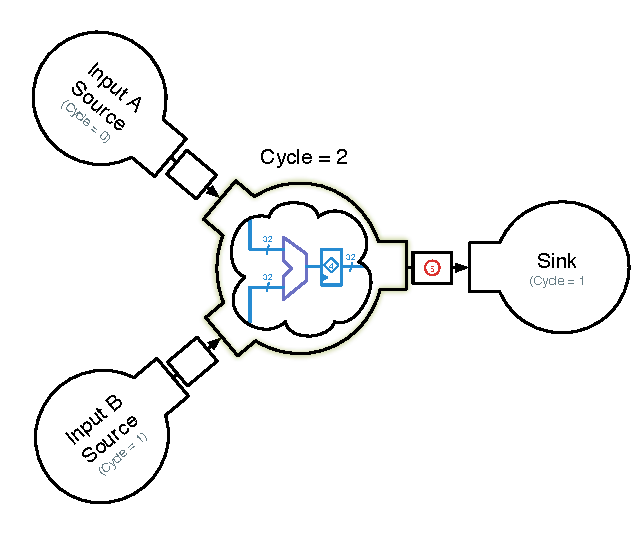
\includegraphics[width=\columnwidth]{figures/adder-example5.pdf}
        \caption{The state of the graph after two firings of the unit.}
        % graffle2pdf -c cycle2 midas-graphics/graffle/adder-example.graffle figures/adder-example5.pdf
    \end{subfigure}
    \centering
    \vspace{-0.25in}
    \caption{A 32-bit adder model and environment simulating a single cycle of target time.}
    \label{fig:adder-example}
\end{figure*}

If the simulation designer uses exclusively, non-wire-type channels both
formalisms are free of deadlock, as there exists no unit whose output at cycle
$t$ depends on the output of another unit also at cycle $t$\footnote{From a
conservative PDES persective, every LP has a non-zero lookahead, and given that
every LP sends messages at every timestamp (obviating the need for null
messages), deadlock is avoided by construction}. In these simulators, all units
can excute cycle $t$ concurrently, which assuming no other sources of delay,
permits the simulator to run at unity FMR.  However, as with latency-insensitive boundaries, it is not always possible to define LP
at registered boundaries.  The use of wire-type channels, (i.e. combinational
coupling between LPs) that introduces two principle challenges: at best, it
increases simulator FMR, and at worst, it may introduce time-0 simulation
deadlock. To illustrate each of these effects, in Figure~\ref{fig:channel-deadlock} we consider a
latency insensitive interface between two units implemented using a queue-type
channel, one pipe and one wire-type channel, and two wire-type channels.

\begin{figure*}
    \centering
    \begin{subfigure}[t]{0.49\textwidth}
        \captionsetup{margin=0.25cm}
        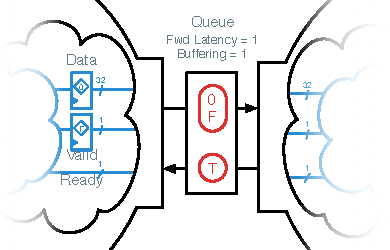
\includegraphics[width=\columnwidth]{figures/li-queue-channel-manual.pdf}
        \caption{A RAMP-style queue-type channel. This allows both models to
        fire simultaenously, but may only be used if it is acceptable to model
        a target queue in the channel.}
        %  -c queue midas-graphics/graffle/deadlock.graffle figures/li-queue-channel.pdf
    \end{subfigure}
    \begin{subfigure}[t]{0.49\textwidth}
        \captionsetup{margin=0.25cm}
        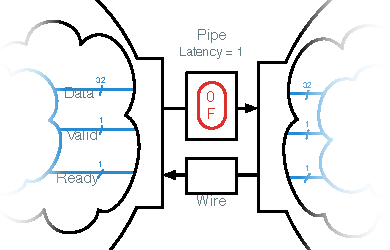
\includegraphics[width=\columnwidth]{figures/li-pipe-channel-manual.pdf}
        \caption{One pipe-type channel, and one-wire type channel carrying the backpressure. This leads $FMR >= 2$, with the consumer unit
        firing first to produce a backpressure token that is subsequently consumed by the producer unit.}
        %  -c pipe midas-graphics/graffle/deadlock.graffle figures/li-pipe-channel.pdf
    \end{subfigure}
    \begin{subfigure}[t]{0.49\textwidth}
        \captionsetup{margin=0.25cm}
        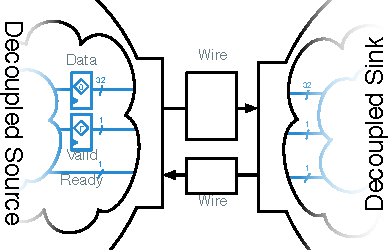
\includegraphics[width=\columnwidth]{figures/li-wire-channel-manual.pdf}
        \caption{Two-wire type channels. This deadlocks an APort Network, as neither producer nor consumer unit can fire
        before the other.}
        % -c wire midas-graphics/graffle/deadlock.graffle figures/li-wire-channel.pdf
    \end{subfigure}
    \centering
    \vspace{-0.25in}
    \caption{Three potential channel modelling decisions for a latency insensitive interface between two units.}
    \label{fig:channel-deadlock}
\end{figure*}

Wire-type channels tend to increase FMR as in general a
combinational path that spans $N$, units will take $N$ cycles to execute, with
other channels connecting these units preventing pipelining of multiple cycles
(i.e., this latency cannot be overlapped, with the simulation of younger target
cycles).

Deadlock is the more pressing challenge. Wire-type channels remove the
aforementioned property that all LPs have non-zero lookahead.  Here there are
two situations that may emerge. If the target itself has a combinational loop,
the behavior of the target is undefined, and simulation deadlock is
unavoidable~\footnote{We note it is possible to have "false" combinational
loops but many tools reject these patterns, and so it's not unreasonable to ban
them in these simulators as well.}. Fortunately, hardware designers know well
to avoid combinational loops. The second challenge arises from poor LP
implementation, such as the simple unit given above, that attempts to enqueue
and dequeue multiple messages atomically. This has the effect of introducing an
extranous combinational dependency between output messages and input messages,
even though there is no combinational path between these outputs and inputs in
the underlying target. We give an example of this in \TODO{figure}. Given its
definition of a unit, APort Networks do not give a sufficient set of
constraints to avoid deadlock as a graph that contains a cycle of wire-type
channels -- that do not represent a combinational loop in the target -- vacuously
deadlocks at time 0.


\subsection{Latency-Insensitive Bounded-Dataflow Networks}

Unlike channel bootstrapped formalisms, LI-BDNs avoid deadlock by imposing
different constraints on the implementation of LPs based on the underlying
hardware they model, and remove the need for specialized channels to bootstrap
simulation. Since connections between LPs always represent wire-like
connectivity in the connectivity LI-BDNs impose no contraints on how the target
is divided into LPs. LI-BDNs were originally developed as a more flexible abstraction for building
latency-sensitive designs that preserve the RTL timing of a synchronous circuit, extending
the work of Carloni et al., in the Theory of Latency Insensitive Design. This problem is analogous
to constructing an ITDC simulator from synchronous ASIC RTL.

In the terms of the paper, what we have loosely referred to as a synchronous
block of RTL is defined synchronous sequential machine~(SSM). Vijayaraghavan et
al.\cite{LIBDN} formally define an SSM:

\begin{widequote}
An SSM is a network of combinational operators or gates
such as AND, OR, NOT, and state elements such as registers,
provided the network does not contain any cycles which has
only combinational elements.
\end{widequote}

Missing from this definition is any treatment of multiple clock domains, differ
types of state elements, asynchronous set or reset.  Inherent to the name
``Synchronous'', Vijayaraghavan et al. forbid their existence -- in an SSM
\emph{all} state updates occur simultaenously. While this limits the
applicability of their approach, much of a modern SoC locally meets this
definition, such as the islands of a GALS-based design.

An LI-BDN is a dataflow network of latency-insensitive nodes whose
edges represent FIFO communication channels with non-zero, but finite (hence,
bounded) capacity. The latency-insensitive nodes of the graph are
referred to as \emph{Primitive LI-BDNs}~(in PDES terms, these are LPs), which is to say, they 
are not themselves subgraphs of more than one node. A
LI-BDN is said to \emph{implement} an SSM, if it \emph{partially implements}
the SSM, and is deadlock free.

In the terms of a hardware engineer, partial implementation~(PI) implies that
the message trace of outputs from the ports of the LI-BDN "matches" the
per-cycle trace of outputs from the SSM. Vijayaraghavan et al.\cite{LIBDN}
formally define PI:

\begin{widequote}
A BDN $R$ partially implements an SSM $S$ iff
\begin{enumerate}
\item There is a bijective mapping between the inputs of $S$ and
[the input tokens of] $R$, and a bijective mapping between the outputs of $S$ and
[the output tokens of] $R$.
\item The output histories of $S$ and $R$ match whenever the
input histories match, i.e.,
\begin{align*}
\forall n &> 0\\
&\text{$I(k)$ for $S$ and $R$ matches $(1 \leq k \leq n)$}\\
\Rightarrow &\text{$O(j)$ for $S$ and $R$ matches $(1 \leq j \leq n)$}
\end{align*}
\end{enumerate}
\end{widequote}

An SSM can be partially implemented in many different ways. For instance, the
LP implementation desribed in \TODO{REF} is a valid partial implementation of
the source RTL. However, it cannot \emph{implement} a larger SSM as it is
susceptible to deadlock when composed with other LPs.  LI-BDNs garauntee
deadlock freedom by adhering to two additional properties. The first, is
\emph{No Extraenous Depedencies}~(NED), which defines when an LP is obligated to enqueue output messages. Vijayaraghavan et al.\cite{LIBDN} formally define NED:

\begin{widequote}
A primitive BDN has the NED property if all output FIFOs have been enqueued at least $n-1$ times,
and for each output $O_i$, all the FIFOs for the inputs in $\emph{CombinationallyConnected}(O_i)$
are enqueued $n$ times, and all other input FIFOs are enqueued at least $n-1$ times, then $O_i$ FIFO
must eventually be enqueued $n$ times.
\end{widequote}\label{def:ned}

% Goes after NED
Intuitively, it exploits the same observation that
permits a pipe-type channel to send output messages before receiving any input
messages could apply to units -- any output channel driven only by state in the
LP (i.e., it's not combinationally coupled to an input) can enqueue an output
messages for cycle $t$ before receiving any input messages for cycle $t$.

The second property an LI-BDN must satisfy is the \emph{self-cleaning}~(SC) property. SC 
defines when an LP is obligated to dequeue input tokens. Vijayaraghavan et al.\cite{LIBDN} formally define SC:

\begin{widequote}
A primitive BDN has the SC property, if when all the
outputs are enqueued $n$ times, all the input FIFOs must
[eventually]\footnote{Clarified in~\cite{LIBDNMasters}.} be dequeued $n$ times, assuming an infinite source for each
input.
\end{widequote}\label{def:sc}

While the nodes of an APort Networks do not always satisfy NED, they do satisfy
SC. At it's heart, SC provides an assurance that LPs drain their input FIFOs,
allowing those FIFOs remain bounded. We note that if and LP fails to satisfy
SC, it will likely fail to partially implement its SSM unless its outputs are
completely independent of the inputs from which it is failing to dequeue. In
this case, having unbounded FIFOs would suffice to prevent deadlock.

Of particular concern to this dissertation, is method through which an SSM can
be converted into an LI-BDN.  Vijayaraghavan et al. describe a means that uses
a wrapper module around the patient SSM based on it's combinational
depedencies. The SSM is treated as a black box otherwise. The wrapper circuit,
for a single output, is shown in \ref{figure}.

This method is highly amenable to automation with a FAME compiler, as it requires
only the ability analyze combinational depedencies in the underlying SSM.

\section{The MIDAS Compiler \& Simulator Microarchitecture}



Two dimensions of classification.

Timekeeping Strategy
% Implicit (Cycle-based) vs Explicit (Time-stamped)

Simulation Control (Spectrum)
% Centralized vs Distributed

Synchronization Schemes \& Control Algorithms
%Synchronization
% Formalisms for Distributed, implicitly time-kept RTL Simulators

MIDAS FAME-1 Transform \& Simulator Microarchitecture

